\documentclass[10pt,letterpaper]{article}

\usepackage[margin=0.7in]{geometry}
\usepackage{graphicx}
\usepackage{booktabs}
\usepackage{tabularx}
\usepackage{xcolor}
\usepackage{hyperref}
\usepackage{enumitem}
\usepackage{parskip}
\usepackage{microtype}
\usepackage{float}
\usepackage{amsmath}
\usepackage{amssymb}
\usepackage{tcolorbox}
\usepackage{pgfplots}
\usepackage{tikz}
\usetikzlibrary{arrows.meta, positioning}
\pgfplotsset{compat=1.18}

\definecolor{primary}{HTML}{1E40AF}
\definecolor{accent}{HTML}{F59E0B}
\definecolor{success}{HTML}{059669}
\definecolor{danger}{HTML}{DC2626}
\definecolor{surface}{HTML}{F1F5F9}
\definecolor{muted}{HTML}{64748B}
\definecolor{border}{HTML}{CBD5E1}

\hypersetup{
  colorlinks=true,
  linkcolor=primary,
  urlcolor=primary,
  pdftitle={Campus Cloud Print Queue Experiments Report},
  pdfauthor={Anand Mohan Singh, Vaibhav Thalanki, Pranav Viswanathan},
}

\newcommand{\code}[1]{\texttt{\small #1}}
\newcommand{\http}[1]{\textbf{\texttt{#1}}}
\setlist[itemize]{noitemsep, topsep=2pt, leftmargin=14pt}
\setlength{\parskip}{4pt}
\setlength{\parindent}{0pt}

\newtcolorbox{claimbox}{
  colback=primary!6,
  colframe=primary!35,
  boxrule=0.5pt,
  arc=2pt,
  left=6pt, right=6pt, top=4pt, bottom=4pt,
}

\newtcolorbox{resultbox}{
  colback=success!8,
  colframe=success!35,
  boxrule=0.5pt,
  arc=2pt,
  left=6pt, right=6pt, top=4pt, bottom=4pt,
}

\newtcolorbox{limitbox}{
  colback=accent!8,
  colframe=accent!35,
  boxrule=0.5pt,
  arc=2pt,
  left=6pt, right=6pt, top=4pt, bottom=4pt,
}

\begin{document}

{\Large\bfseries Campus Cloud Print Queue: Experiments and Results\par}
{\small CS 6650 Final Project --- Northeastern University\par}
{\small Anand Mohan Singh, Vaibhav Thalanki, Pranav Viswanathan\par}

\vspace{4pt}
\begin{tcolorbox}[colback=surface,colframe=border,boxrule=0.5pt,arc=2pt,left=6pt,right=6pt,top=4pt,bottom=4pt]
\textbf{System under test.} Campus Cloud Print Queue is a release-at-device printing platform with a stateless Go Gin API on ECS Fargate, DynamoDB conditional writes for job state, S3 for document storage, and one SQS queue plus one worker per printer. The experiments test four core claims: horizontal API scaling, lock-free correctness under contention, queue isolation under overload, and crash recovery through SQS redelivery plus idempotent workers.
\end{tcolorbox}

\textbf{Experimental framing.} The four experiments were chosen to cover both \textit{performance} and \textit{correctness} tradeoffs in the system design. Experiment 1 measures throughput and latency for the stateless API tier. Experiment 2 validates that concurrent releases are serialized correctly at the storage layer. Experiment 3 studies backlog behavior when one printer is overloaded. Experiment 4 injects a worker failure to verify end-to-end recovery.

\textbf{Why these experiments matter.} Together, these runs cover the most failure-prone parts of the architecture: request bursts at the API edge, race conditions on shared state, overload localized to one printer, and crashes during in-flight work. The report therefore emphasizes evidence for design choices rather than raw benchmark volume alone.

\section*{Experiment 1: API Load Test}
\begin{claimbox}
\textbf{Purpose / tradeoff.} We evaluated \textbf{stateless horizontal scaling} vs.\ stateful routing. A stateless API simplifies deployment and failover, but only if externalized state in DynamoDB and S3 does not become the bottleneck.
\end{claimbox}

\textbf{Method.} Locust (\code{tests/experiment1\_load\_test/locustfile.py}) ran a mixed workload at 50 concurrent users for 120 seconds against the public ALB. Traffic included uploads, status polling, list operations, release, delete, health checks, and negative-path validation requests. Because requests are distributed through the load balancer, the run also implicitly exercises the assumption that any API task can serve any request without sticky session state.

\begin{table}[H]
\centering
\caption{Experiment 1 summary}
\begin{tabularx}{\linewidth}{@{}lX@{}}
\toprule
\textbf{Metric} & \textbf{Value} \\
\midrule
Total requests & 4,891 \\
Errors & 16 total, all HTTP 429 on \http{POST /jobs} \\
Error rate & 0.33\% \\
Effective throughput & \textasciitilde25 req/s \\
Slowest endpoint & \http{POST /jobs}: 120 ms p50, 440 ms p99 \\
Fastest endpoint & \http{DELETE /jobs/{id}}: 95 ms p50 \\
\bottomrule
\end{tabularx}
\end{table}

\begin{table}[H]
\centering
\caption{Experiment 1 endpoint latency percentiles (ms)}
\begin{tabular}{@{}lrrrr@{}}
\toprule
\textbf{Endpoint} & \textbf{Requests} & \textbf{p50} & \textbf{p95} & \textbf{p99} \\
\midrule
\http{GET /health}         & 1100 & 100 & 100 & 120 \\
\http{POST /jobs}          &  489 & 120 & 200 & 440 \\
\http{GET /jobs}           & 1310 & 110 & 130 & 210 \\
\http{GET /jobs/{id}}      &  489 & 110 & 140 & 200 \\
\http{DELETE /jobs/{id}}   &  390 &  95 & 120 & 120 \\
\http{POST /release}       &  390 & 110 & 140 & 210 \\
\http{POST /release (bad)} &  131 &  92 & 110 & 120 \\
\http{GET /user/{id}}      &  489 &  94 & 110 & 120 \\
\http{GET /user/status}    &  103 &  94 & 120 & 210 \\
\bottomrule
\end{tabular}
\end{table}

\begin{figure}[H]
\centering
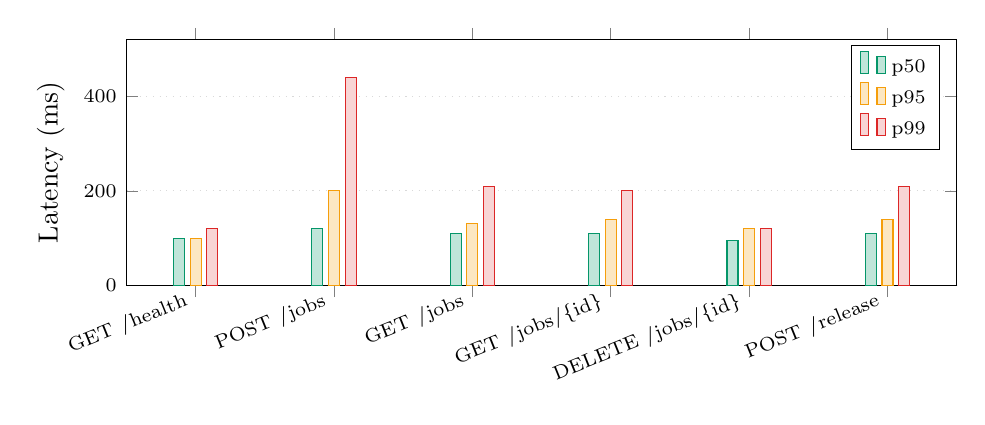
\begin{tikzpicture}
\begin{axis}[
  ybar,
  bar width=4pt,
  width=\linewidth,
  height=4.7cm,
  ylabel={Latency (ms)},
  symbolic x coords={GET /health, POST /jobs, GET /jobs, GET /jobs/\{id\}, DELETE /jobs/\{id\}, POST /release},
  xtick=data,
  x tick label style={rotate=22, anchor=east, font=\scriptsize},
  legend style={at={(0.98,0.98)},anchor=north east,font=\scriptsize},
  ymin=0, ymax=520,
  ymajorgrids=true,
  grid style={dotted,gray!30},
  tick label style={font=\scriptsize},
]
\addplot[fill=success!25, draw=success] coordinates {
  (GET /health,100) (POST /jobs,120) (GET /jobs,110) (GET /jobs/\{id\},110)
  (DELETE /jobs/\{id\},95) (POST /release,110)
};
\addplot[fill=accent!25, draw=accent] coordinates {
  (GET /health,100) (POST /jobs,200) (GET /jobs,130) (GET /jobs/\{id\},140)
  (DELETE /jobs/\{id\},120) (POST /release,140)
};
\addplot[fill=danger!20, draw=danger] coordinates {
  (GET /health,120) (POST /jobs,440) (GET /jobs,210) (GET /jobs/\{id\},200)
  (DELETE /jobs/\{id\},120) (POST /release,210)
};
\legend{p50, p95, p99}
\end{axis}
\end{tikzpicture}
\caption{Response time percentiles by endpoint}
\end{figure}

\begin{resultbox}
\textbf{Analysis.} The API handled nearly 4.9k requests with no 5xx failures, which supports the stateless design claim. Uploads were the slowest path because they include S3 writes, while read-heavy endpoints stayed in the 100--200 ms p99 range. The small number of 429s indicates controlled overload rather than instability.

The data also shows that the externalized-state design is working as intended. DynamoDB-backed reads and conditional state transitions remained well below half a second even under mixed traffic, while the more expensive S3 upload path explains the heavier tail on \http{POST /jobs}. This separation matters because it means horizontal API scaling is not being undermined by lock contention or in-memory coordination between tasks.
\end{resultbox}

\begin{limitbox}
\textbf{Limitations.} This was a single 50-user run. We did not search for the saturation point of the API layer or run longer tests to measure sustained queue-depth effects.
\end{limitbox}

\section*{Experiment 2: DynamoDB Contention Test}
\begin{claimbox}
\textbf{Purpose / tradeoff.} We tested \textbf{optimistic concurrency with DynamoDB conditional writes} against the alternative of distributed locking. The question was whether exactly-one-release semantics can be enforced without introducing a lock service.
\end{claimbox}

\textbf{Method.} Using \code{tests/experiment2\_contention/contention\_test.py}, we created one \texttt{HELD} job per trial and fired concurrent release requests at levels $N \in \{2,5,10,20,50\}$ using \code{asyncio.gather}. The expected result was exactly one HTTP 200 and $N-1$ HTTP 409 responses. All requests targeted the same job ID so the storage layer was forced to arbitrate a true write-write race.

The API handler implements the release transition with a DynamoDB conditional update on \code{status = HELD}. In the full service, that update also sets \code{printerName} and increments a version counter. The experiment therefore directly tests the core correctness primitive used by the production release path, rather than a mocked approximation.

\begin{table}[H]
\centering
\caption{Experiment 2 results}
\begin{tabular}{@{}rrrrr@{}}
\toprule
\textbf{N} & \textbf{200} & \textbf{409} & \textbf{Errors} & \textbf{Avg Latency (ms)} \\
\midrule
2  & 1 & 1  & 0 & 185 \\
5  & 1 & 4  & 0 & 183 \\
10 & 1 & 9  & 0 & 197 \\
20 & 1 & 19 & 0 & 196 \\
50 & 1 & 49 & 0 & 346 \\
\bottomrule
\end{tabular}
\end{table}

\begin{figure}[H]
\centering
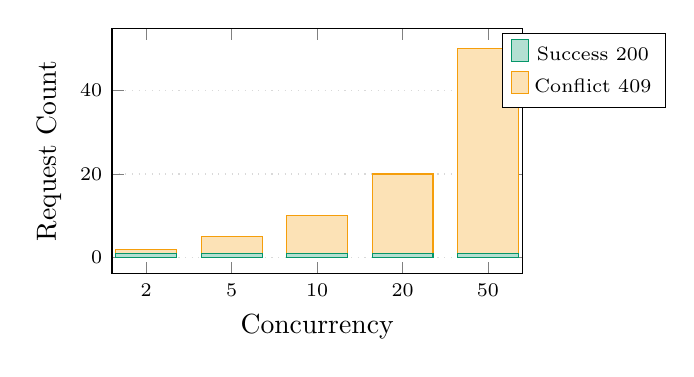
\begin{tikzpicture}
\begin{axis}[
  ybar stacked,
  bar width=22pt,
  width=0.56\linewidth,
  height=4.7cm,
  xlabel={Concurrency},
  ylabel={Request Count},
  symbolic x coords={2,5,10,20,50},
  xtick=data,
  legend style={at={(1.35,0.98)},anchor=north east,font=\scriptsize},
  ymajorgrids=true,
  grid style={dotted,gray!30},
  tick label style={font=\scriptsize},
]
\addplot[fill=success!30,draw=success] coordinates {(2,1)(5,1)(10,1)(20,1)(50,1)};
\addplot[fill=accent!30,draw=accent] coordinates {(2,1)(5,4)(10,9)(20,19)(50,49)};
\legend{Success 200, Conflict 409}
\end{axis}
\end{tikzpicture}
\hfill
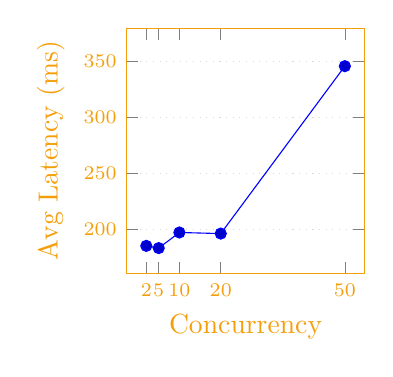
\begin{tikzpicture}
\begin{axis}[
  width=0.38\linewidth,
  height=4.7cm,
  xlabel={Concurrency},
  ylabel={Avg Latency (ms)},
  xtick={2,5,10,20,50},
  ymin=160, ymax=380,
  ymajorgrids=true,
  grid style={dotted,gray!30},
  tick label style={font=\scriptsize},
  mark=*,
  color=accent,
]
\addplot coordinates {(2,185)(5,183)(10,197)(20,196)(50,346)};
\end{axis}
\end{tikzpicture}
\caption{Exactly-one-wins behavior under concurrent release attempts}
\end{figure}

\begin{resultbox}
\textbf{Analysis.} Every run produced the intended result: one success, the rest clean conflicts, and no errors. This is strong evidence that the DynamoDB conditional write is sufficient to enforce release exclusivity without locks. Latency increased only moderately even at 50 simultaneous writers, suggesting correctness is preserved without introducing a major coordination penalty.

This result is especially important because the system allows releases to arrive from multiple clients without session affinity. If correctness depended on application-level locking, failures such as lock leakage, lock timeout tuning, or crashed lock owners would become new operational risks. Here, the storage layer provides the serialization guarantee directly.
\end{resultbox}

\begin{limitbox}
\textbf{Limitations.} Each test used one hot key at a time. We did not combine contention with broader production-like background load or measure behavior when SQS send fails after the write succeeds.
\end{limitbox}

\section*{Experiment 3: Printer Saturation Test}
\begin{claimbox}
\textbf{Purpose / tradeoff.} We studied \textbf{per-printer queues} vs.\ a single global queue. Per-printer queues cost slightly more SQS resources, but should isolate one slow or overloaded printer from the others.
\end{claimbox}

\textbf{Method.} The saturation client in \code{tests/experiment3\_saturation/saturation\_test.py} created 50 jobs and release-attempted them concurrently to \code{printer-1}. The worker processes one job at a time with a simulated 5--15 second service time. The script records completion counts and latency for jobs that reach \texttt{DONE}. This setup mirrors the real physical constraint of a single printer handling one document at a time, so the queue acts as the shock absorber for bursty demand.

This setup intentionally creates a service-rate mismatch: the client can submit work much faster than one worker can drain it. That makes it useful for observing whether overload manifests as controlled queue growth and higher wait time, or as corruption, loss, or unstable behavior.

\begin{table}[H]
\centering
\caption{Experiment 3 summary}
\begin{tabularx}{\linewidth}{@{}lX@{}}
\toprule
\textbf{Metric} & \textbf{Value} \\
\midrule
Jobs submitted (upload attempted) & 50 \\
Jobs accepted by upload API & 50 \\
Jobs completed (DONE) within polling window & 23 \\
Jobs still incomplete at timeout & 27 \\
Release status breakdown & Not persisted by the script \\
Min end-to-end latency & 83.4 s \\
Mean end-to-end latency & 350.5 s \\
p50 latency & 395.6 s \\
p95 / p99 latency & 396.1 s \\
\bottomrule
\end{tabularx}
\end{table}

\begin{figure}[H]
\centering
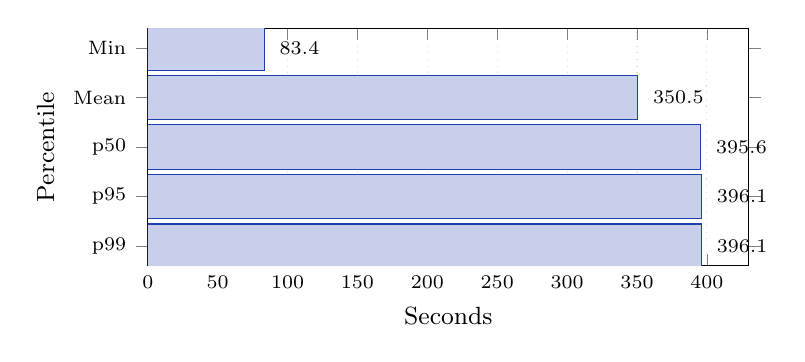
\begin{tikzpicture}
\begin{axis}[
  xbar,
  bar width=16pt,
  width=0.76\linewidth,
  height=4.6cm,
  xlabel={Seconds},
  ylabel={Percentile},
  symbolic y coords={p99, p95, p50, Mean, Min},
  ytick=data,
  xmajorgrids=true,
  grid style={dotted,gray!30},
  tick label style={font=\scriptsize},
  label style={font=\small},
  xmin=0, xmax=430,
  nodes near coords,
  every node near coord/.append style={font=\scriptsize, xshift=2pt},
]
\addplot[fill=primary!25,draw=primary] coordinates {
  (396.1,p99)(396.1,p95)(395.6,p50)(350.5,Mean)(83.4,Min)
};
\end{axis}
\end{tikzpicture}
\caption{Latency growth under single-printer saturation}
\end{figure}

\begin{resultbox}
\textbf{Analysis.} The completed jobs show classic backlog behavior: once the queue fills, end-to-end latency becomes dominated by wait time rather than processing time. The tight clustering near 396 seconds indicates a steady drain rate, which is exactly what we expect from one worker servicing one printer queue. The experiment therefore supports the claim that overload becomes queueing delay instead of silent loss.

This experiment also reinforces the architectural reason for per-printer queues. With a single global queue, jobs for a healthy printer could sit behind a long run of jobs targeting a saturated device. By isolating each printer behind its own queue, overload remains local to that printer's backlog instead of turning into a system-wide head-of-line blocking problem.
\end{resultbox}

\begin{limitbox}
\textbf{Limitations.} The script does not persist per-job release status codes or live queue-depth snapshots, so some intermediate states must be inferred. We also tested only one printer at a time rather than flooding all printers concurrently.
\end{limitbox}

\section*{Experiment 4: Fault Injection and Recovery}
\begin{claimbox}
\textbf{Purpose / tradeoff.} We evaluated \textbf{Standard SQS plus application-level idempotency} against FIFO queues with built-in deduplication. The design goal was to tolerate worker crashes without duplicate printing or manual intervention.
\end{claimbox}

\textbf{Method.} Using \code{tests/experiment4\_fault\_injection/fault\_injection\_test.py}, we released 8 jobs to \code{printer-3}, waited 10 seconds, force-stopped the printer ECS task, and then polled until recovery completed. The mechanism under test was ECS task replacement plus SQS redelivery plus the worker's idempotent reprocessing branch. This is an end-to-end failure test rather than a unit-level simulation, because it depends on the interaction of multiple AWS services.

The recovery path relies on three components cooperating correctly: ECS keeps the service at \code{desired\_count=1}, SQS makes the in-flight message visible again after the visibility timeout expires, and the worker recognizes the \texttt{PROCESSING}+\code{receiveCount > 1} case as a crash-recovery path rather than a duplicate that should be discarded.

\begin{table}[H]
\centering
\caption{Experiment 4 results}
\begin{tabularx}{\linewidth}{@{}lX@{}}
\toprule
\textbf{Metric} & \textbf{Value} \\
\midrule
Jobs released to printer-3 & 8 \\
In PROCESSING state at kill time & 1 \\
Remaining in queue (RELEASED) & 7 \\
ECS restart time & \textasciitilde30 s \\
SQS visibility timeout & 60 s \\
Total recovery time (kill $\to$ all DONE) & 140.5 s \\
Duplicate DONE events & 0 \\
Stuck jobs (never DONE) & 0 \\
FAILED jobs & 0 \\
Final state: 8 / 8 DONE & \textcolor{success}{\checkmark} \\
\bottomrule
\end{tabularx}
\end{table}

\begin{figure}[H]
\centering
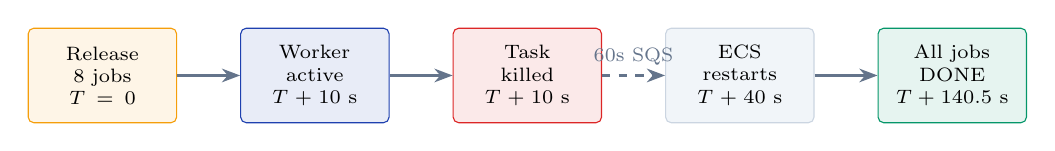
\begin{tikzpicture}[
  phase/.style={
    rectangle, draw=border, fill=surface, rounded corners=2pt,
    minimum width=1.75cm, minimum height=1.2cm, font=\scriptsize, align=center,
    text width=1.65cm,
  },
  arrow/.style={-Stealth, thick, color=muted},
]
\node[phase, draw=accent, fill=accent!10] (release) {Release\\8 jobs\\$T=0$};
\node[phase, draw=primary, fill=primary!10, right=0.8cm of release] (proc) {Worker\\active\\$T+10$ s};
\node[phase, draw=danger, fill=danger!10, right=0.8cm of proc] (kill) {Task\\killed\\$T+10$ s};
\node[phase, right=0.8cm of kill] (restart) {ECS\\restarts\\$T+40$ s};
\node[phase, draw=success, fill=success!10, right=0.8cm of restart] (done) {All jobs\\DONE\\$T+140.5$ s};
\draw[arrow] (release) -- (proc);
\draw[arrow] (proc) -- (kill);
\draw[arrow, dashed] (kill) -- (restart) node[midway, above, font=\scriptsize]{60s SQS};
\draw[arrow] (restart) -- (done);
\end{tikzpicture}
\caption{Recovery timeline after worker termination}
\end{figure}

\begin{resultbox}
\textbf{Analysis.} Recovery completed automatically with no duplicates and no stuck jobs. The dominant delay was the SQS visibility timeout, not ECS restart time, which shows where the real recovery budget sits. This experiment supports the architectural choice to rely on at-least-once delivery plus idempotent state transitions rather than FIFO-only correctness.

The result is also consistent with the broader concurrency strategy used throughout the system. The same style of conditional state transition used in the API release path appears again in the worker's \code{mark\_done} write. That means the correctness story is not split across unrelated mechanisms: API concurrency and worker crash recovery both rely on storage-backed idempotent transitions.
\end{resultbox}

\begin{limitbox}
\textbf{Limitations.} We injected only one failure and killed the worker while one job was in \texttt{PROCESSING}. A harsher test would repeatedly kill the worker or target the exact moment a \code{mark\_done} write is in flight.
\end{limitbox}

\section*{Overall Evidence}
\begin{tcolorbox}[colback=surface,colframe=border,boxrule=0.5pt,arc=2pt,left=6pt,right=6pt,top=4pt,bottom=4pt]
\textbf{What the experiments collectively show.} The evidence supports the main architectural decisions of the project. The API remained stable under mixed traffic without relying on in-memory state. DynamoDB conditional writes enforced exactly-one-release semantics under concurrent access. Per-printer queues converted overload into bounded backlog growth instead of cross-printer interference. Finally, worker crashes were recovered automatically through ECS replacement, SQS redelivery, and idempotent state transitions. The strongest remaining gaps are broader stress ranges, richer instrumentation during saturation, and more adversarial repeated-failure scenarios.
\end{tcolorbox}

\end{document}
